\chapter{Demonstration Problem: Hypersonic Retro-firing Annular Jet}
\label{chapter-five}

To demonstrate the advantages and the robustness of the decoupled flow and
adjoint solvers relative to the fully coupled flow and adjoint solvers, a
demonstration problem is chosen with sufficiently difficult physics.  The
problem must include a sufficient degree of chemistry to highlight the stability
concerns of the decoupled flow solver presented in
\sref{sec:15-kps-sphere-cone}.  This chapter details the geometry and test
conditions of demonstration problem, as well as the characteristics of the flow
solution.

\section{Annular Jet Configuration and Test Conditions}

The geometry chosen is a hypersonic re-entry vehicle with a retro-firing annular
nozzle, as shown in \fref{fig:annular-jet-side}.
%------------------------------------------------------------------------------%
\begin{figure}[h]
  \centering
	\begin{subfigure}[b]{0.4\textwidth}
    \centering
    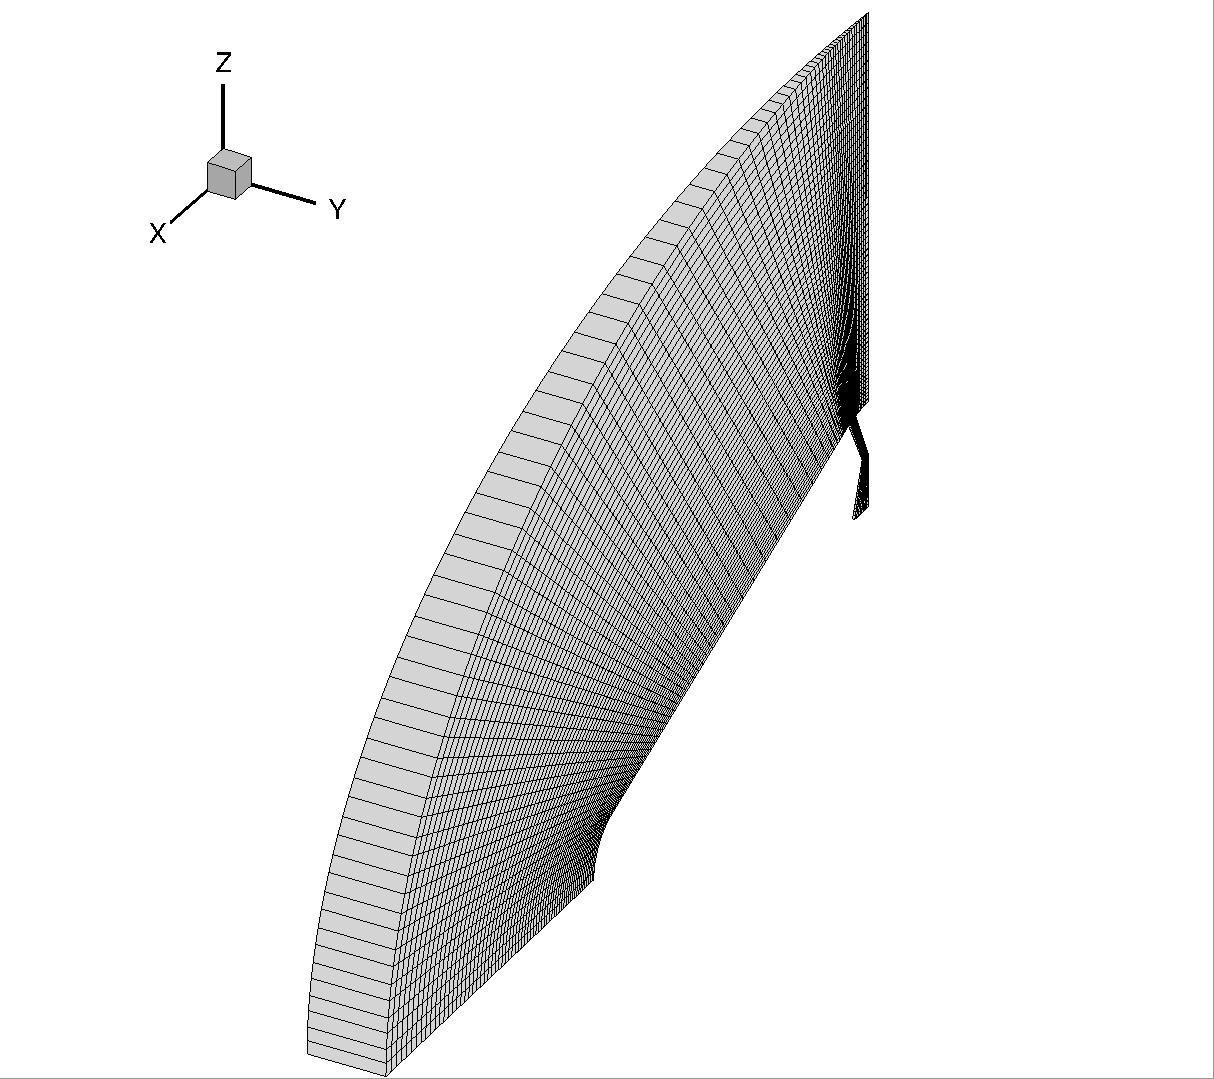
\includegraphics[width=\textwidth]{figures/all_iso.png}
  \end{subfigure}
	\begin{subfigure}[b]{0.4\textwidth}
    \centering
    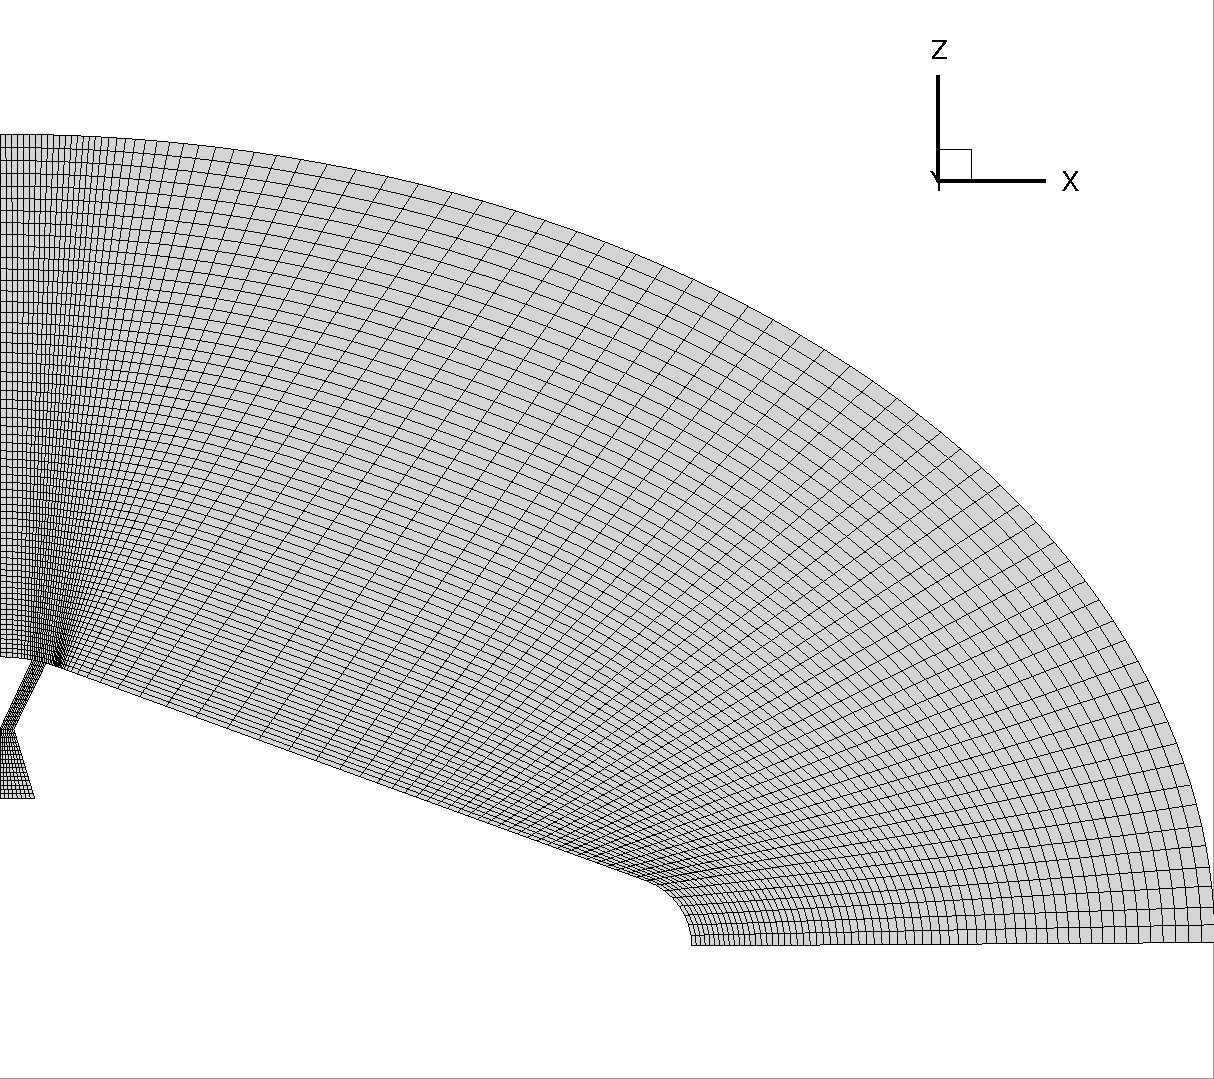
\includegraphics[width=\textwidth]{figures/all_side.png}
  \end{subfigure}
  \caption{Annular Jet Geometry}
  \label{fig:annular-jet-side}
\end{figure}
%------------------------------------------------------------------------------%
This geometry was originally investigated by Gnoffo et
al\cite{gnoffo2016tapping} to obtain increased drag from ``pulsing'' the annular
jet to obtain a beneficial effect from the unsteady shock interaction with the
plume of the jet.  It was also determined from the aforementioned work that a
steady solution to the euler equations exists for this annular jet
configuration.  This problem is attractive for optimization, because the annular
jet plenum conditions significantly affect aerodynamic and aerothermodynamic
quantities of interest on the vehicle surface.  These effects are very
non-linear, due to the shock and jet plume interaction, and it is therefore very
difficult to intuitively understand the relationship between the plenum
conditions and vehicle surface quantities.  Because the adjoint solver is
rigorously derived from the discretized governing equations, the relationship
between the plenum and surface can be directly determined, making this an
excellent showcase problem for adjoint-based sensitivity information.

The geometry was generated with the parameters shown in \tref{tab:annular-geom},
with the mesh originally created as structured grid and then converted to an
unstructured grid of hexahedra elements.
%------------------------------------------------------------------------------%
\begin{table}[h]
  \centering
  \begin{tabular}{c|c|c}
    Parameter & Description & Value \\
    \hline
    $r_{throat}$       &   nozzle throat radius, $m$                 & 0.02 \\
    $r_{plenum,inner}$ &   inside nozzle radius at plenum face, $m$  & 0.02 \\
    $r_{plenum,outer}$ &   outside nozzle radius at plenum face, $m$ & 0.07 \\
    $r_{exit,inner}$   &   inside nozzle radius at exit, $m$         & 0.064 \\
    $r_{exit,outer}$   &   outside nozzle radius at exit, $m$        & 0.08 \\
    $l_{conv}$         &   distance from plenum to throat, $m$       & 0.05 \\
    $\theta_c$         &   cone half angle, deg                      & 50.0
  \end{tabular}
  \caption{Annular Nozzle Geometry Inputs}
  \label{tab:annular-geom}
\end{table}
%------------------------------------------------------------------------------%
The flow conditions are shown in \tref{tab:flow-conditions}
%------------------------------------------------------------------------------%
\begin{table}[!h]
  \centering
  \begin{tabular}{c|c|c}
    Flow Condition & Description & Value \\
    \hline
    $V_{\infty}$    & freestream velocity, $m/s$        & 5686.24 \\
    $\rho_{\infty}$ & freestream density, $kg/m^3$      & 0.001 \\
    $T_{\infty}$    & freestream temperature, $K$       & 200.0 \\
    $M_{\infty}$    & freestream Mach number (derived)  & 20.0
  \end{tabular}
  \caption{Flow Conditions}
  \label{tab:flow-conditions}
\end{table}
%------------------------------------------------------------------------------%

\section{Steadiness Dependence on Cone Angle}

While the reacting gas path of the FUN3D flow solver has the capability to
simulate unsteady flows, the newly developed FUN3D reacting gas adjoint solver
is limited in scope to steady flows only at this time.  A full design
optimization covers a wide variety of flow solutions, and it is therefore
important to verify that the geometry chosen is truly steady.  It was
heuristically determined that blowing a light gas with a high cone angle leads
to a sonic corner body.  A similar phenomenon was examined by Gnoffo,
Weilmuenster, Braun, and Cruz\cite{gnoffo1996influence} for the Mars Pathfinder
probe on descent into the Martian atmosphere.
%------------------------------------------------------------------------------%
\begin{figure}[h]
  \centering
  \begin{subfigure}[b]{0.45\textwidth}
    \centering
    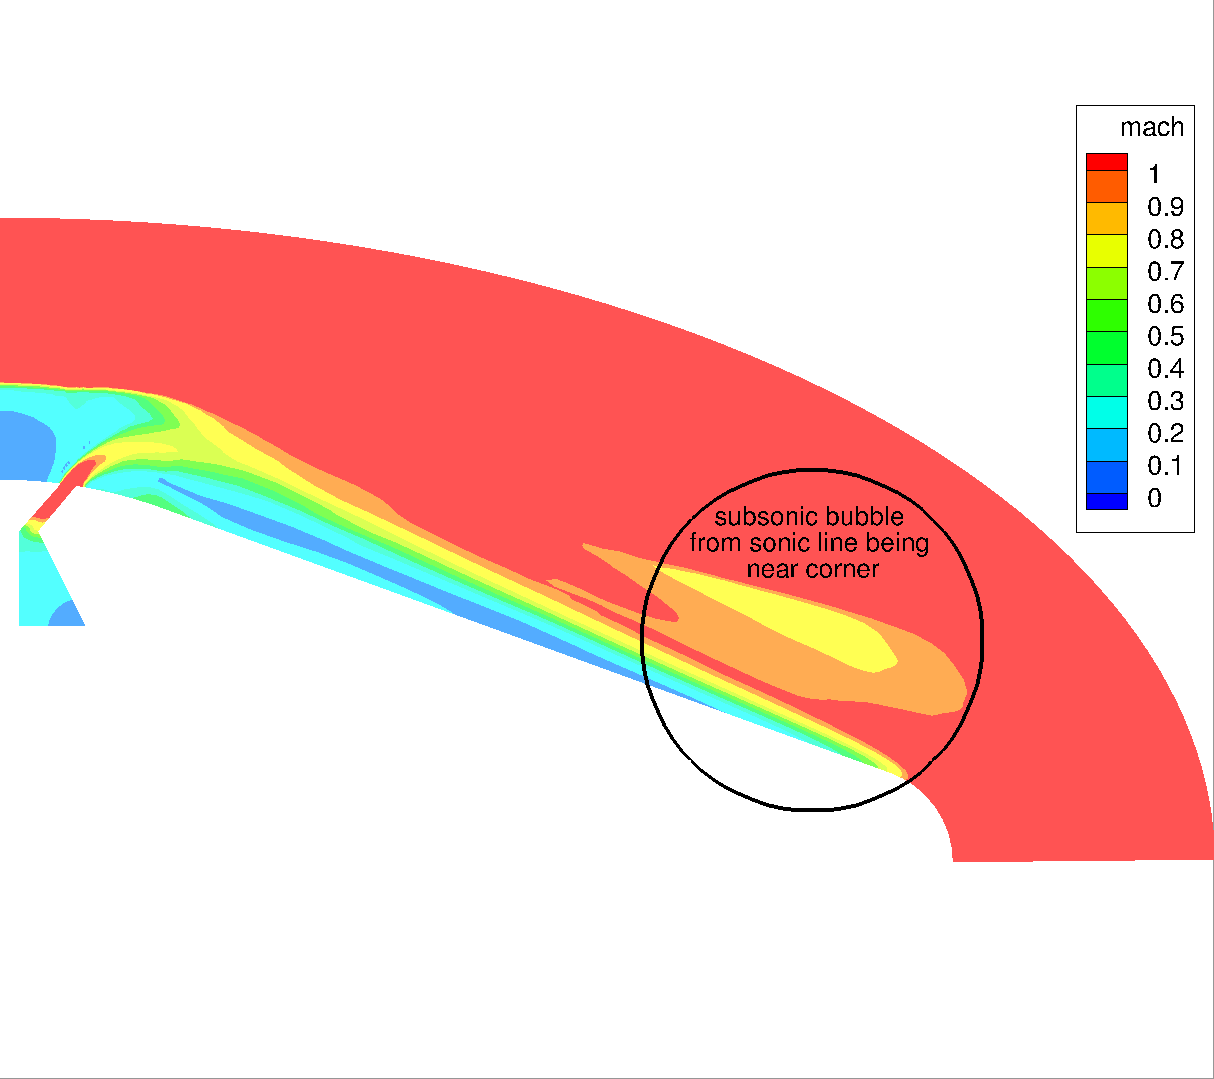
\includegraphics[width=\textwidth]{figures/sonic-bubble/sonic_bubble.png}
    \caption{$70^o$ Cone angle blowing pure $H_2$}
    \label{fig:70-deg-cone}
  \end{subfigure}
  \begin{subfigure}[b]{0.45\textwidth}
    \centering
    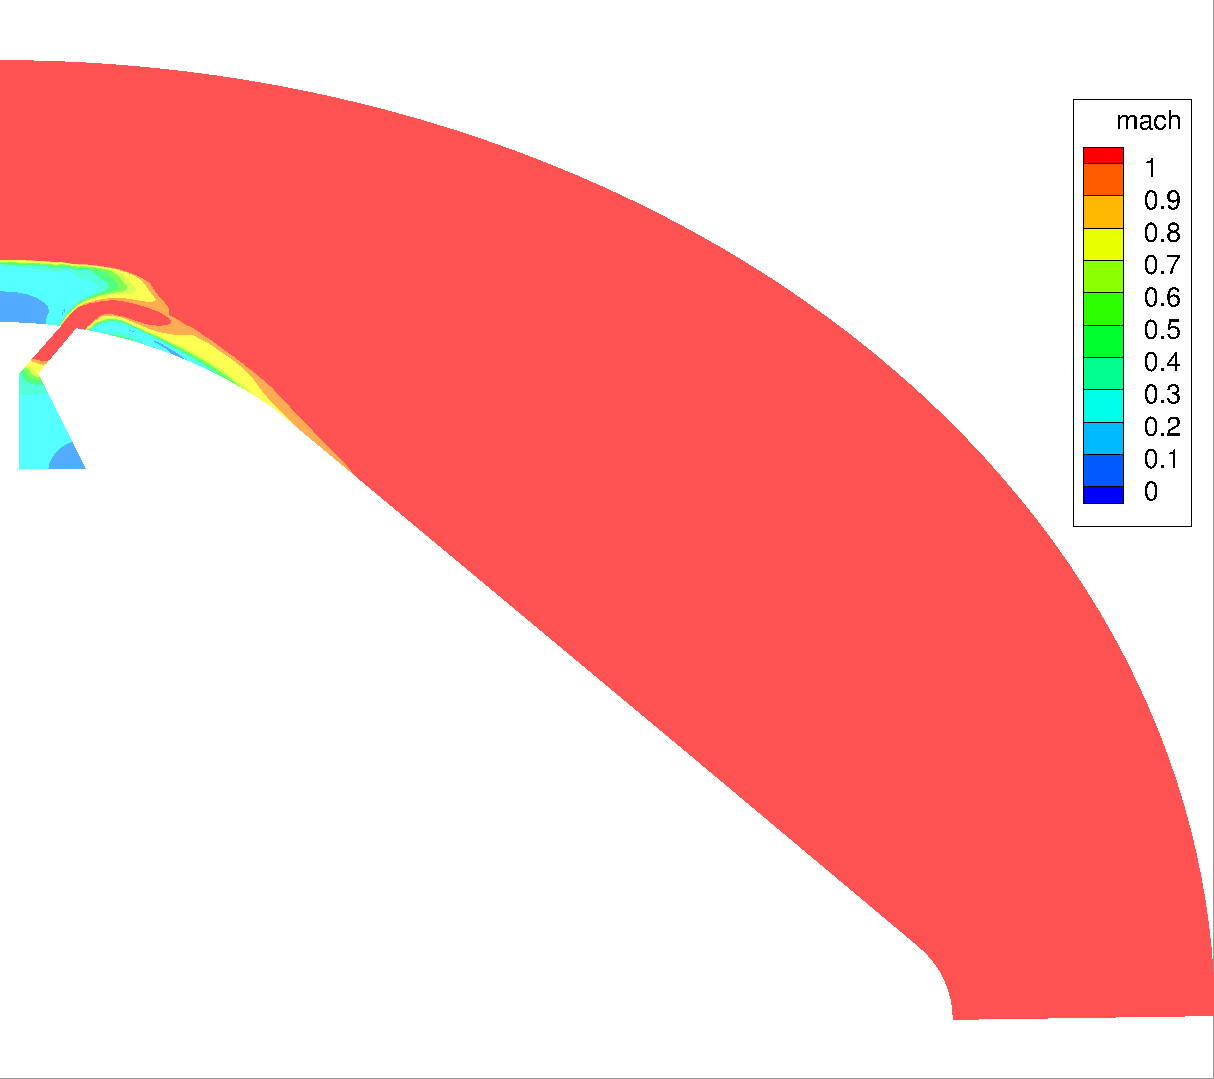
\includegraphics[width=\textwidth]{figures/sonic-bubble/no_bubble.png}
    \caption{$50^o$ Cone angle blowing pure $H_2$}
    \label{fig:50-deg-cone}
  \end{subfigure}
  \caption{Cone angle comparison}
  \label{fig:cone-angle-comp}
\end{figure}
%------------------------------------------------------------------------------%
\fref{fig:cone-angle-comp} shows a comparison of blowing pure $H_2$ from the
plenum on a vehicle with a $50^o$ cone angle and $70^o$ cone angle.
\fref{fig:70-deg-cone} highlights the subsonic bubble that is indicative of a
sonic corner body, whereas \fref{fig:50-deg-cone} shows that decreasing the cone
angle moves the sonic line upstream and eliminates the subsonic bubble.  The
strong dependence between the position of the sonic line on the vehicle and the
cone angle is the primary reason that the cone angle was chosen to be decreased
to $50^o$, rather that using the $70^o$ chosen by
Gnoffo\cite{gnoffo2016tapping}.  The comparision between the $50^o$ and
$70^o$ cone angle geometries was done for a wide range of plenum conditions
spanning the design space to be discussed in the next chapter, and no subsonic
bubble was ever found for the $50^o$ cone angle.

\section{Mesh Refinement Study}

To determine the flow solution mesh sensitivity, a grid convergence study was
attempted by uniformly refining the original mesh, using the cut-cell method
developed by Park\cite{???} that uniformly divides each element in the mesh.
\fref{fig:mesh-refined} shows the progression of refined meshes generated by
this method
%------------------------------------------------------------------------------%
\begin{figure}[h]
  \centering
  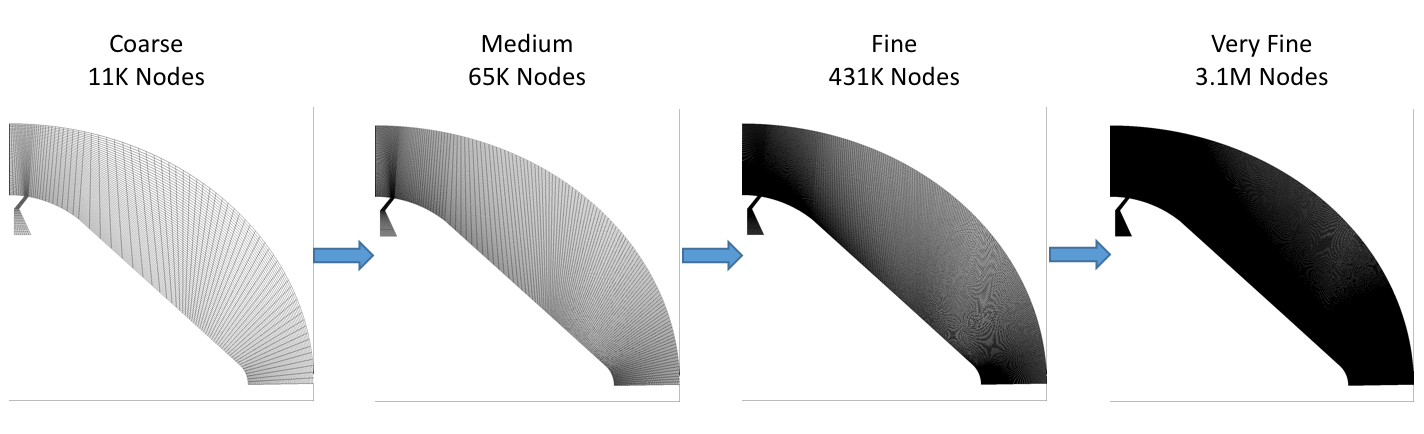
\includegraphics[width=\textwidth]{figures/mesh-progression.png}
  \caption{Uniformly Refined Meshes}
  \label{fig:mesh-refined}
\end{figure}
%------------------------------------------------------------------------------%
\fref{fig:grid-convergence} shows the grid convergence of surface temperature
and plenum mass flow rate for a nominal case.
%------------------------------------------------------------------------------%
\begin{figure}[h]
  \centering
  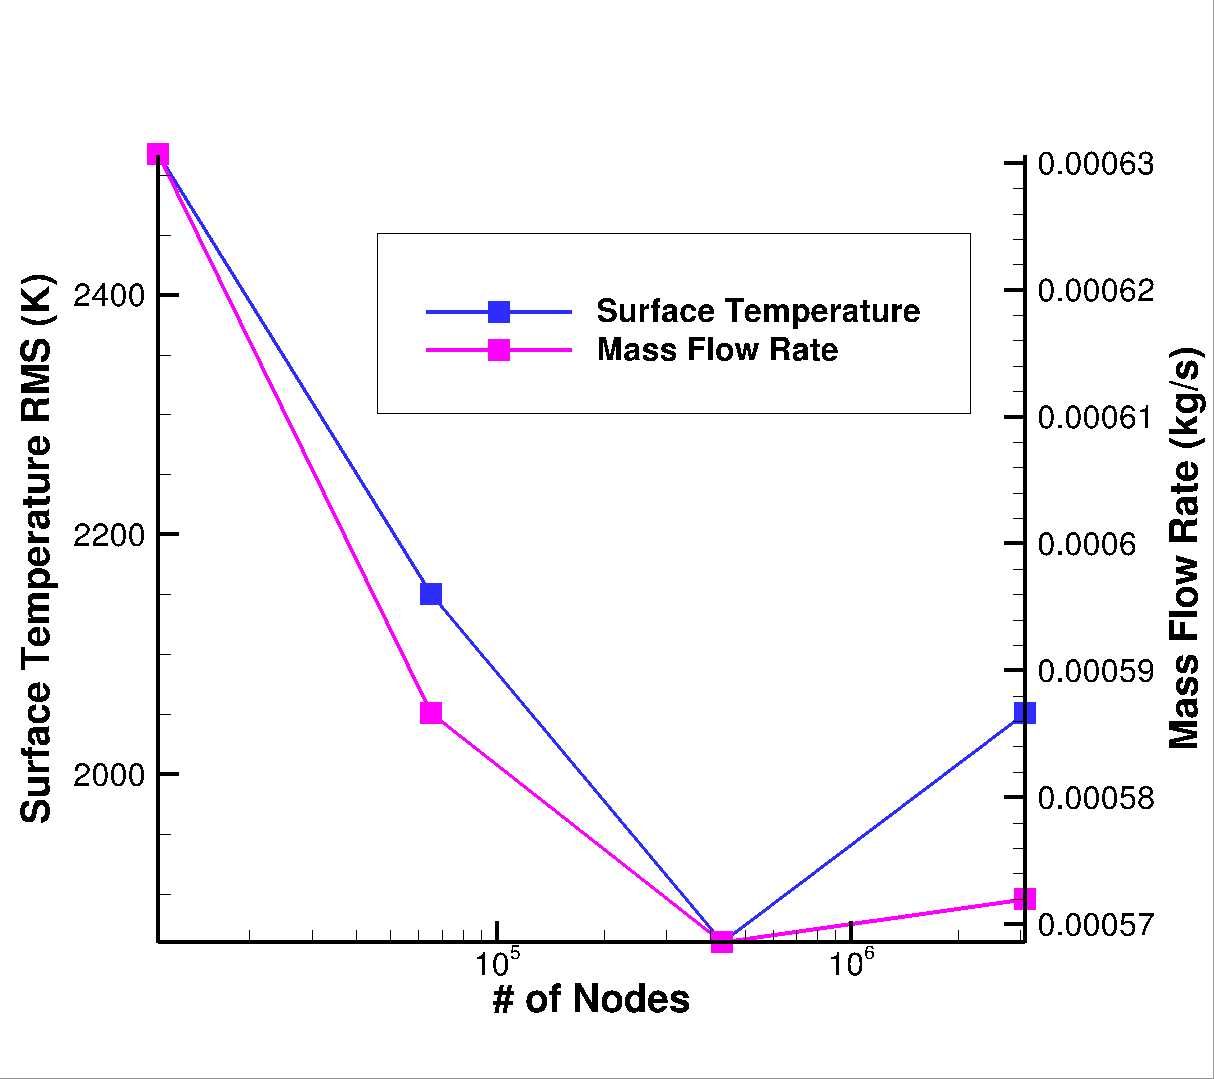
\includegraphics[width=0.5\textwidth]{figures/t-m-conv.png}
  \caption{Grid convergence }
  \label{fig:grid-convergence}
\end{figure}
%------------------------------------------------------------------------------%
the fine mesh ($431,000$ Nodes) was found to be slightly unsteady, but coerced
to be steady when the limiter was frozen.  The very fine mesh was very unsteady,
and freezing the flux limiter did not coerce the flow back to steady.  The
values for surface temperature and mass flow rate on the very fine mesh are time
averaged quantities presented for qualitative purposes only.  This grid
convergence study shows that the demonstration problem resolves to unsteadiness
on a fine enough mesh.  For the purposes of demonstrating the decoupled
discrete adjoint, the discretized flow solution must remain steady; therefore,
the coarse mesh ($11,000$ nodes) is used for the remainder of this study, with
the caveat that the grid converged flow solution is truly an unsteady problem.

